\chapter{Evaluation}

This chapter goes through the experiments conducted to simulate various artwork transportation scenarios, building upon the experiments in Section 4.6. Due to connectivity challenges outlined in Chapter 5.2, modifications were made to facilitate these experiments using local implementations.

\section{Experiment 0}

Experiment 0 is the basis for these experiments, it shows the measured data of the board staying 28 hours on a table. While temperature and humidity might change, the acceleration has to be almost non-existent for the board to be accurate.

The experiment was conducted following these steps:

\begin{enumerate}
\item Connect the board (USB ST-LINK) to the laptop using a USB micro cable.
\item Launch Tera Term, select 'Serial' and choose 'COM3: STMicroelectronics STLink Virtual COM Port (COM3)' as the 'Port'.
\item Adjust the baud rate to 115200 under 'Setup' > 'Serial Port...' in Tera Term.
\item Log data with timestamps using 'File' > 'Log...' in Tera Term.
\item Execute the 'Temperature' project on the board.
\item Run TeraTermPlot.py, specifying the log file name and location chosen in step 4.
\item Place the setup on a table and leave it like that for 28 hours.
\item Stop data plotting after 28 hours and proceed to analyze the collected data.
\end{enumerate}

\begin{figure}[H]
\centering
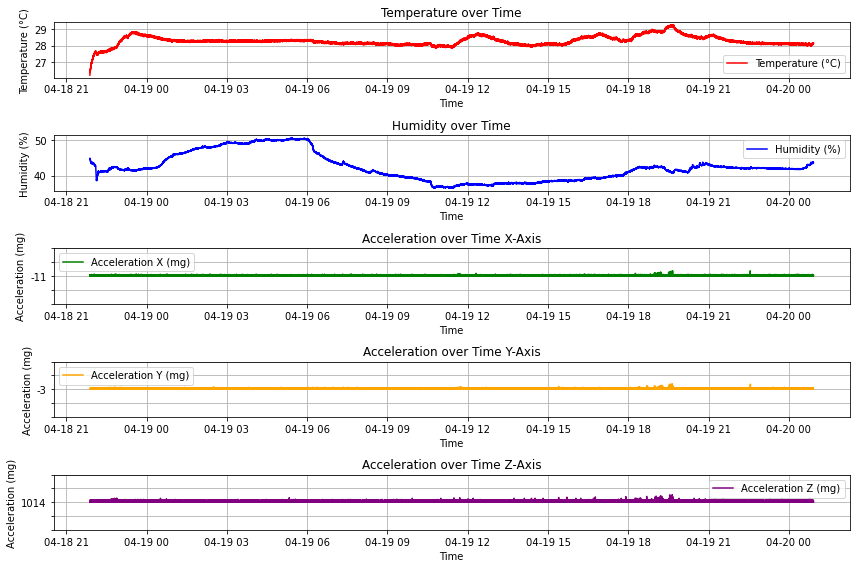
\includegraphics[width=1\linewidth]{plot_exp_0.png}
\caption{Environmental Data Experiment 0}
\label{fig:Environmental Data Experiment 0}
\end{figure}

As shown in Figure 6.1, both temperature and humidity changed during the 28 hours. One reason for the humidity change between 04-19 00 and 04-19 06 was the presence of a sleeping person in the room during that period.
Throughout the 28 hours, the acceleration across all three axes remained constant. The X- and Y-axes recorded values of -11 mg and -3 mg, respectively, indicating minimal acceleration close to zero on these axes. The Z-axis, however, showed an acceleration of 1014 mg, with some slight movement caused by the usage of the table, over the 28 hours, nearly aligning with the expected value of around 1000 mg when the sensor is oriented parallel to the Earth's surface. This alignment corresponds to Earth's gravity, which is approximately 1000 mg.
This experiment also demonstrates that the system is capable of functioning effectively during extended transportation durations, which is frequently encountered in real-world scenarios.

\section{Experiment 1}

Experiment 1 tested local communication between the ST-Board and a laptop, measuring the system's temperature, humidity, and acceleration. It also tested the system's reliability in a dynamic scenario, such as going on a walk.

\begin{figure}[H]
    \centering
    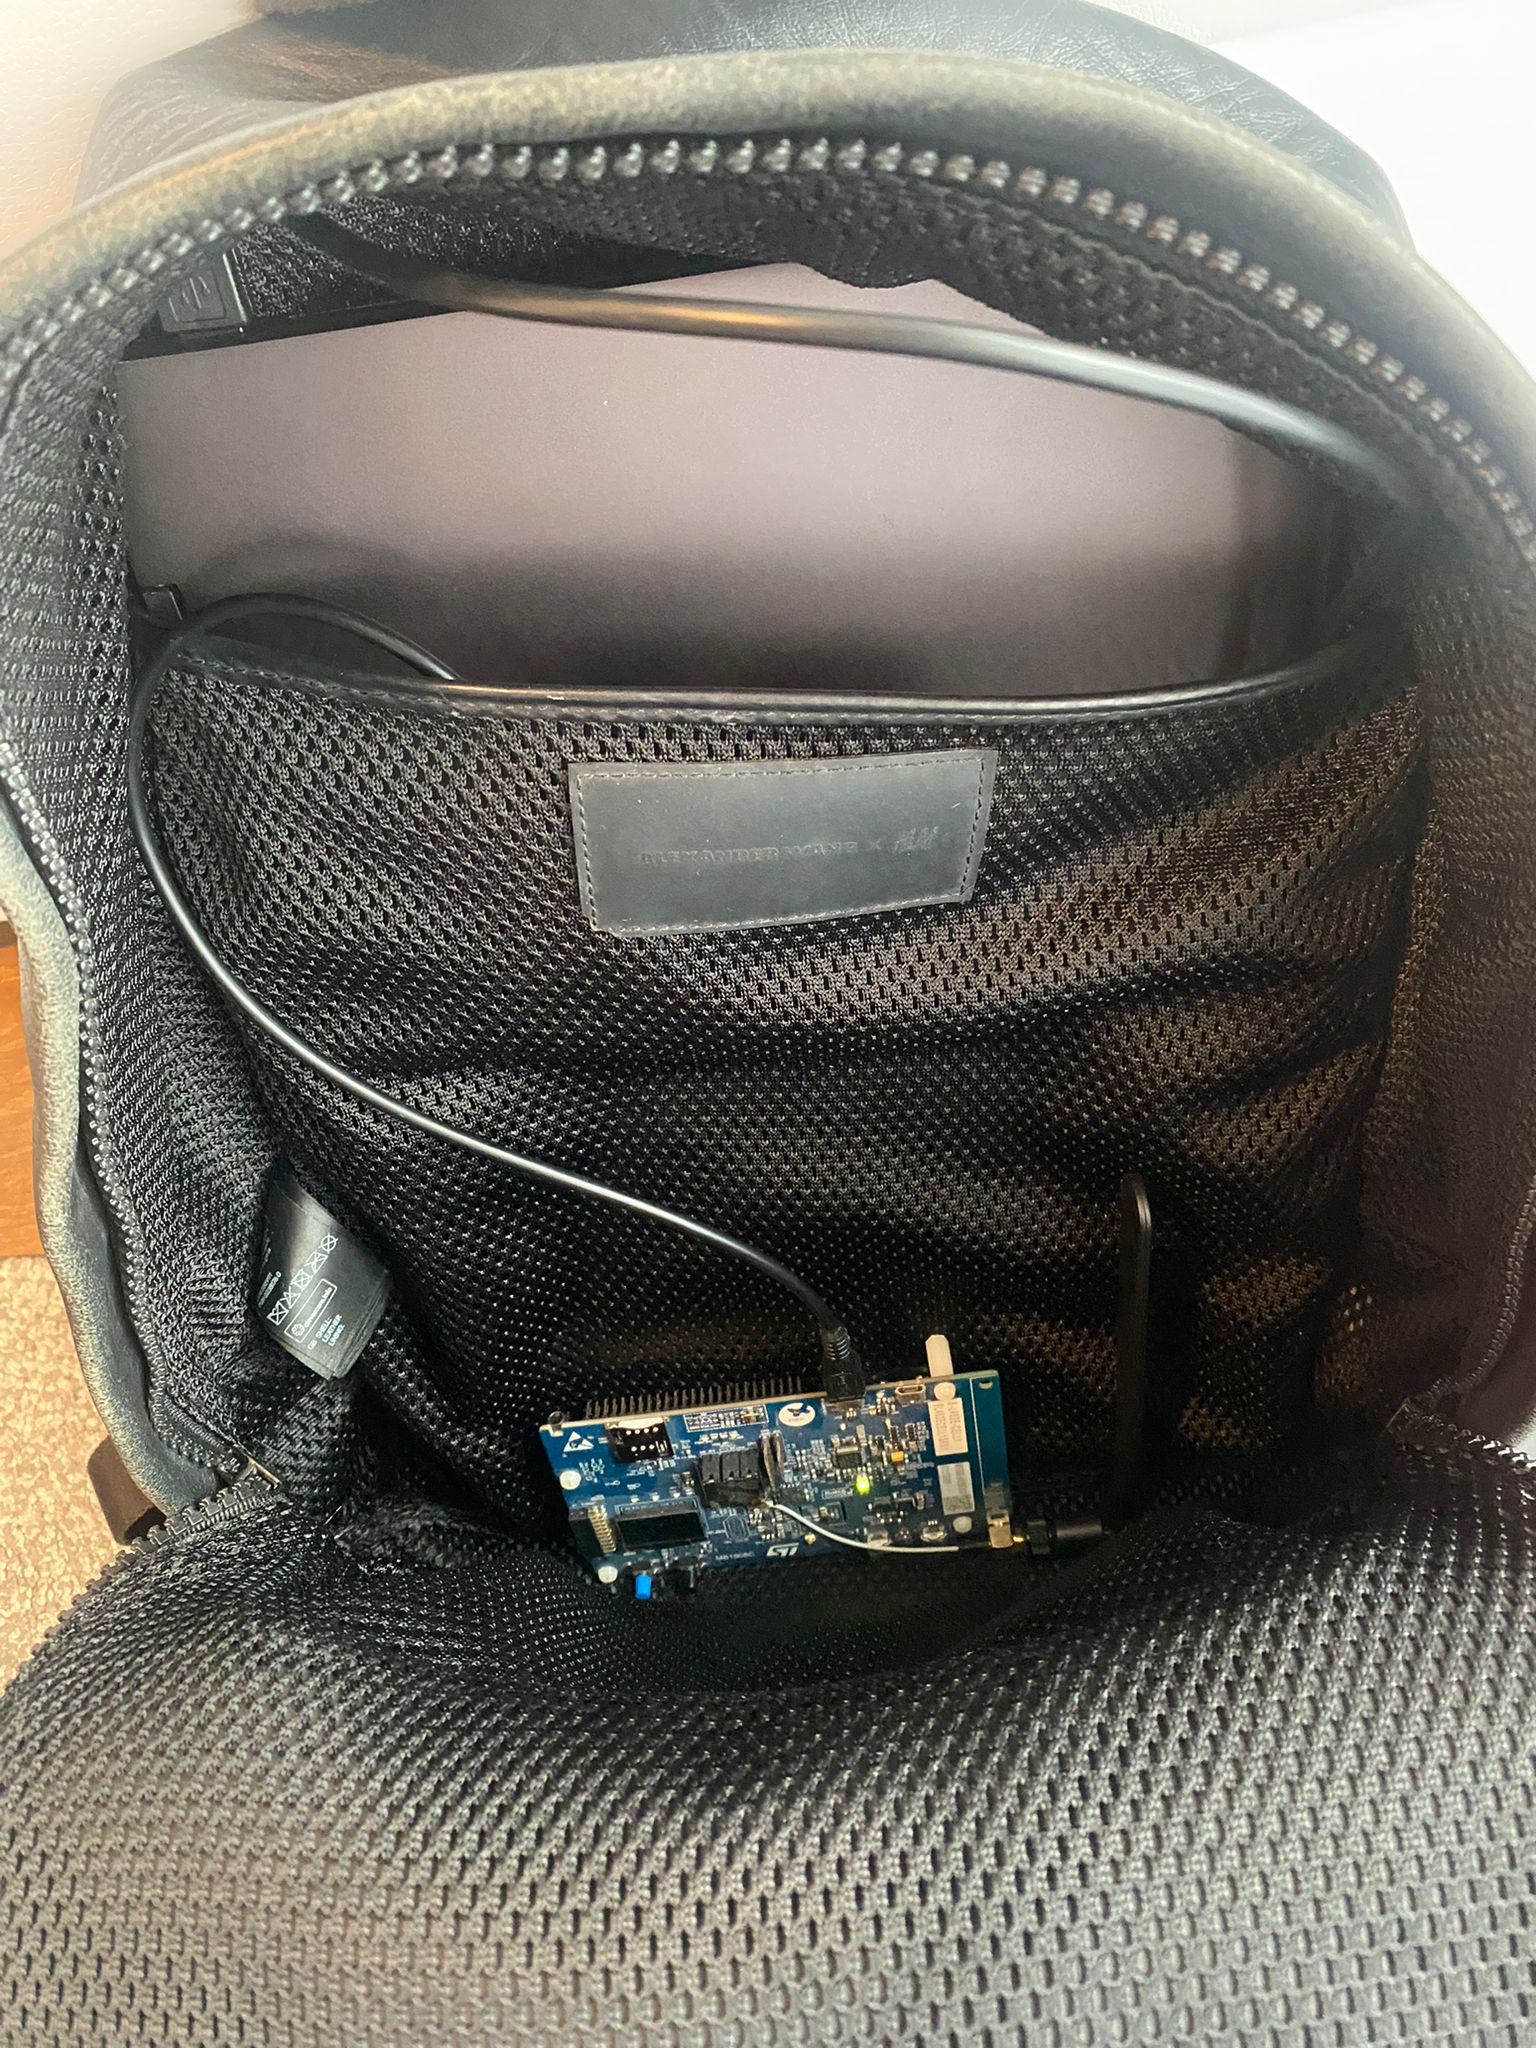
\includegraphics[width=0.5\linewidth]{Backpack_Experiment_1.jpeg}
    \caption{Backpack scenario}
    \label{fig:Backpack scenario}
\end{figure}

The experiment was conducted following these steps:

\begin{enumerate}
\item Connect the board (USB ST-LINK) to the laptop using a USB micro cable.
\item Launch Tera Term, select 'Serial' and choose 'COM3: STMicroelectronics STLink Virtual COM Port (COM3)' as the 'Port'.
\item Adjust the baud rate to 115200 under 'Setup' > 'Serial Port...' in Tera Term.
\item Log data with timestamps using 'File' > 'Log...' in Tera Term.
\item Execute the 'Temperature' project on the board.
\item Run TeraTermPlot.py, specifying the log file name and location chosen in step 4.
\item Place the setup in a backpack as shown in Figure 6.2 and walk the designated route (see Figure 4.3).
\item Stop data plotting at the end of the walk and proceed to analyze the collected data.
\end{enumerate}

\begin{figure}[H]
\centering
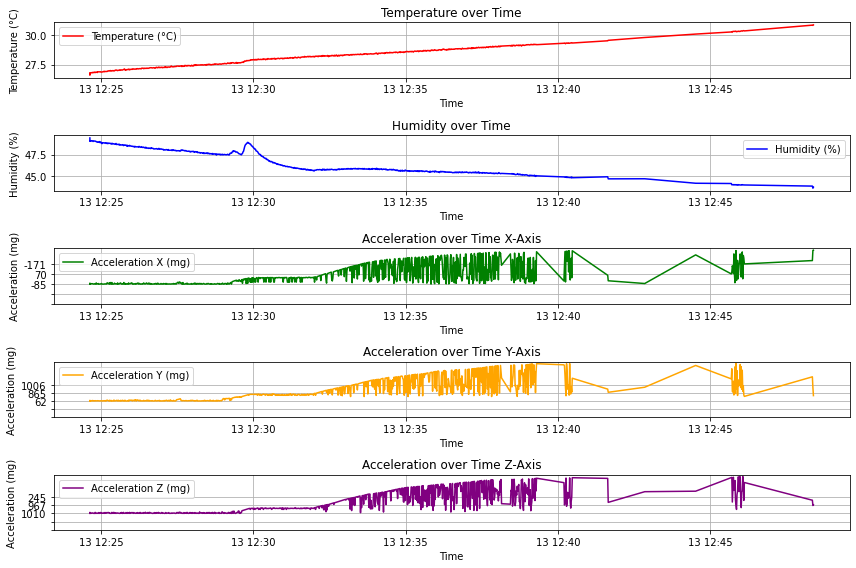
\includegraphics[width=1\linewidth]{plot_exp_1.png}
\caption{Environmental Data Experiment 1}
\label{fig:Environmental Data Experiment 1}
\end{figure}

As shown in Figure 6.3 the temperature rose during the walk. The reason for that was the direct sunlight on the backpack, which also led to the humidity drop throughout the walk.

\section{Experiment 2}

Experiment 2 expanded on local communication and data measurement by testing the system in a faster scenario. To test that, the system was put into a car, giving insights into its performance under faster conditions.

The experiment procedure included:

\begin{enumerate}
\item Connecting the board (USB ST-LINK) to the laptop using a USB micro cable.
\item Initiating Tera Term, selecting 'Serial' and choosing 'COM3: STMicroelectronics STLink Virtual COM Port (COM3)' as the 'Port'.
\item Setting the baud rate to 115200 under 'Setup' > 'Serial Port...' in Tera Term.
\item Logging data with timestamps using 'File' > 'Log...' in Tera Term.
\item Running the 'Temperature' project on the board.
\item Executing TeraTermPlot.py with the specified log file name and location from step 4.
\item Placing the setup within the car and driving the designated route (see Figure 4.4).
\item Stopping data plotting at the end of the drive and proceeding to analyze the collected data.
\end{enumerate}

\subsection{Experiment 2a}

\begin{figure}[H]
\centering
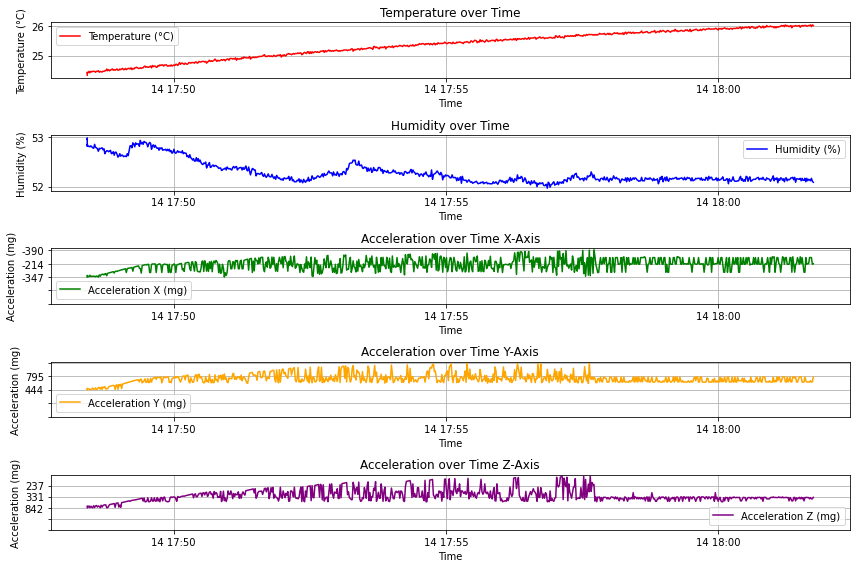
\includegraphics[width=1\linewidth]{plot_exp_2a.png}
\caption{Environmental Data Experiment 2a}
\label{fig:Environmental Data Experiment 2a}
\end{figure}

In Figure 6.4 the temperature showed a slight increase during the drive, rising from 24.5 degrees to 26 degrees. The humidity remained relatively stable, fluctuating between 53\% and 52\%. The acceleration data showed consistent patterns throughout the ride, without any longer pauses or significant fluctuations.

\subsection{Experiment 2b}
A second experiment was conducted under similar conditions. The only difference was an open window for 6 minutes during the ride. This allowed for the investigation of how external factors can influence the data.

\begin{figure}[H]
\centering
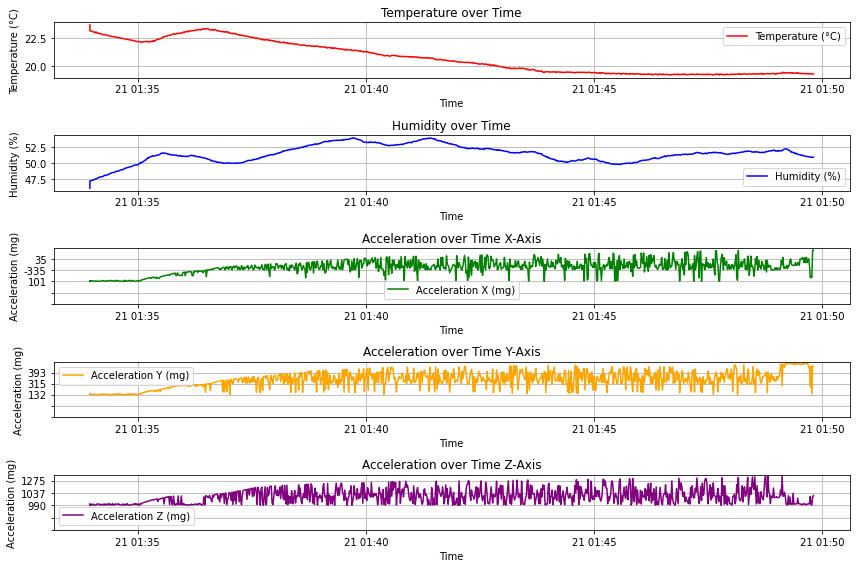
\includegraphics[width=1\linewidth]{plot_exp_2b.png}
\caption{Environmental Data Experiment 2b}
\label{fig:Environmental Data Experiment 2b}
\end{figure}

Figure 6.5 shows a temperature drop between 21 01:37 and 21 01:43 from 23.4 degrees to 19.8 degrees, due to the open window during that period. The humidity had more fluctuation than in Experiment 2a going from 47.5\% up to 53\%. The acceleration looks similar to the first drive with a little bit more fluctuation and a longer stop at around 21 01:36 due to a construction site.

\section{Experiment 3}

Experiment 3 combined elements from experiments 1 and 2 and introduced additional challenges, such as using public transportation like buses and trains. It also tests the reliability of the system in a metal container.

The experiment followed these steps:

\begin{enumerate}
\item Connecting the board (USB ST-LINK) to the laptop using a USB micro cable.
\item Opening Tera Term, selecting 'Serial' and choosing 'COM3: STMicroelectronics STLink Virtual COM Port (COM3)' as the 'Port'.
\item Setting the baud rate to 115200 under 'Setup' > 'Serial Port...' in Tera Term.
\item Logging data with timestamps using 'File' > 'Log...' in Tera Term.
\item Running the 'Temperature' project on the board.
\item Executing TeraTermPlot.py with the specified log file name and location from step 4.
\item Placing the setup in a backpack and following these steps:
\begin{enumerate}
\item Walking to the train station.
\item Taking the train.
\item Changing to a bus.
\item Leaving the bus and completing the designated route (see Figure 4.5) by walking.
\end{enumerate}
\item Stopping data plotting at the end of the route and proceeding to analyze the collected data.
\end{enumerate}

\subsection{Experiment 3 Fail}

\begin{figure}[H]
    \centering
    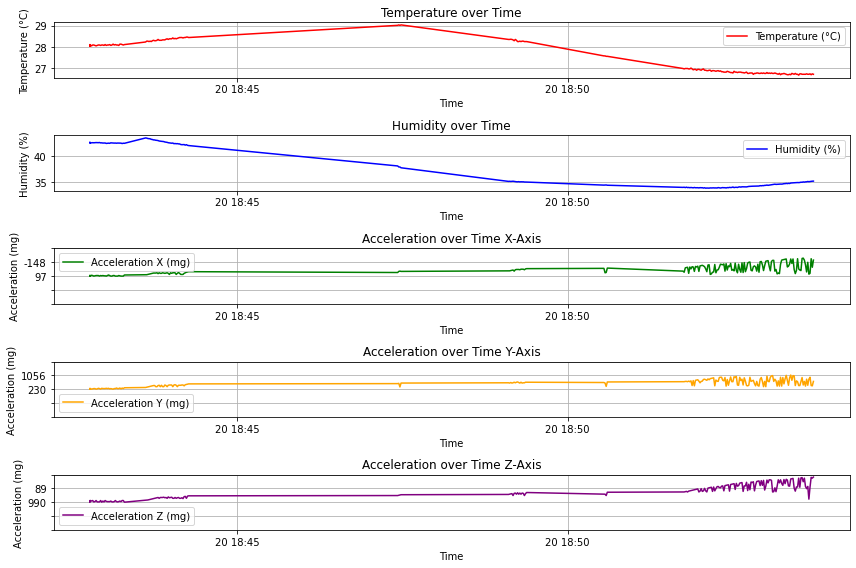
\includegraphics[width=1\linewidth]{plot_exp_3_fail.png}
    \caption{Failed Environmental Data Experiment 3}
    \label{fig:Failed Environmental Data Experiment 3}
\end{figure}

The initial attempt failed after 10 minutes. The board disconnected during the transport, due to movement of the cable inside the bag.

\subsection{Experiment 3 Second Attempt}

\begin{figure}[H]
    \centering
    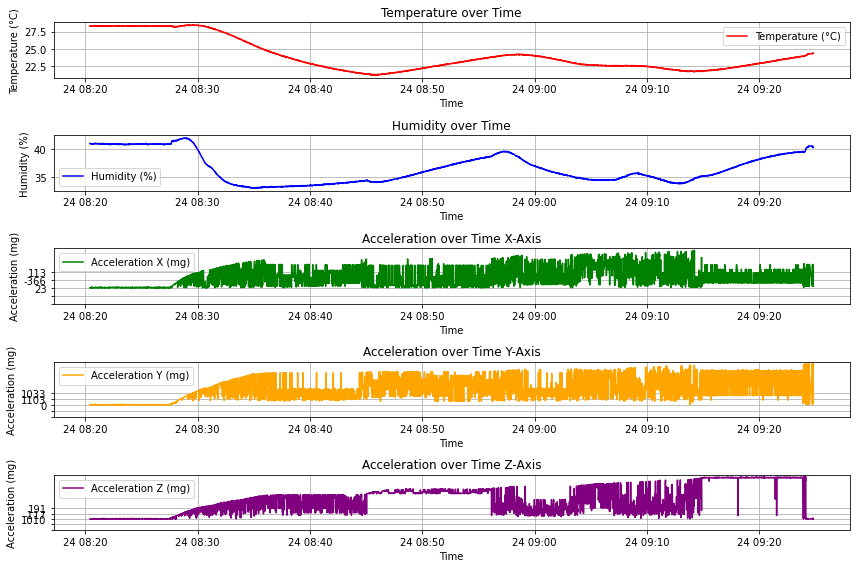
\includegraphics[width=1\linewidth]{plot_exp_3.png}
    \caption{Environmental Data Experiment 3}
    \label{fig:Environmental Data Experiment 3}
\end{figure}

On the second attempt data collection worked. Various transportation methods can be seen using the data. Initially, from 24 08:28 to 24 08:45, the board was transported on foot, exhibiting acceleration data similar to Experiment 1. At the same time, there was a decrease in temperature and humidity. Subsequently, from 24 08:45 to 24 08:56, the board was transported by train, showcasing reduced z-axis fluctuations, and a rise in temperature and humidity during the ride. Following this, from 24 08:57 to 24 09:03, another walking phase was conducted before switching to bus transport until 24 09:07. The final leg of the journey was again on foot.

\section{Discussion}
Even Though it was not possible to implement the planned system as a whole, due to connectivity challenges, adaptations were made to test data measurement and local logging in different scenarios.
The lack of documentation for the board made the implementation of data sensing more challenging. However, despite this hurdle, the system exhibited consistent transmission during all experiments, showcasing its reliability in local communication. The only point of failure identified was the cable disconnecting, which can be addressed by using a bigger backpack.
The system proved capable of capturing environmental data accurately, even in faster-paced situations like car and train transportation. This shows that the prototype can reliably function in the real-world art transport environment.
It also proved to be useful for a longer transport as shown in experiment 0, where the system worked for 28 hours without any problem.

Table 6.1 gives an overview of the different experiments that were conducted. It shows that all 4 Experiments tested the connection between the board and laptop, and they all tested if the data was measured correctly. Experiments 1, 2, and 3 also tested if the system works in dynamic situations, whereas Experiments 2 and 3 also tested if there is a difference if the system moves faster. Moreover, Experiment 3 explored the impact of being in a metal container, like a train, on the accuracy of the data. Experiment 0 also tested if the system works for a longer period.


\begin{table}[H]
    \centering
    \begin{tabular}{c|c|c|c|c|c|c}
        & Connection & Measurement& Dynamic & Speed & Container & Longer Duration\\
        \hline
        Experiment 0 & $\surd$ & $\surd$ & X & X & X & $\surd$\\
        \hline
        Experiment 1 & $\surd$ & $\surd$ & $\surd$ & X & X & X\\
        \hline
        Experiment 2 & $\surd$ & $\surd$ & $\surd$ & $\surd$ & X & X\\
        \hline
        Experiment 3 & $\surd$ & $\surd$ & $\surd$ & $\surd$ & $\surd$ & X\\
    \end{tabular}
    \caption{Experiments Overview Evaluation}
    \label{tab:Experiments Overview Evaluation}
\end{table}